\documentclass[10pt,sigconf,anonymous]{acmart}

\usepackage{booktabs} % For formal tables
\usepackage{atbegshi}% http://ctan.org/pkg/atbegshi
\AtBeginDocument{\AtBeginShipoutNext{\AtBeginShipoutDiscard}}
\usepackage{tabu}
\usepackage{upgreek}
\usepackage{amsthm}
\usepackage[inline]{enumitem}
\usepackage{xcolor}
\usepackage{commath}
\usepackage{graphicx}
\graphicspath{{C:/Users/melli/OneDrive/UOITPhDResearch/anomaly-model-v4/images/}}
\usepackage[linesnumbered,commentsnumbered,boxed]{algorithm2e} 
\usepackage{multicol}
\usepackage{multirow}
\usepackage{bm}
\usepackage{units}
\usepackage{amsmath,amssymb,latexsym}
\numberwithin{equation}{section}
\usepackage{url}
\usepackage{algorithmic}
\usepackage{array}
\usepackage{epstopdf}
\usepackage{hhline}
\usepackage[T1]{fontenc}
\usepackage[caption=false]{subfig}
\renewcommand{\baselinestretch}{1.03}


\begin{document}
\copyrightyear{2019} 
\acmYear{2019} 
\setcopyright{acmcopyright}
\acmConference[LCTES 2019]{LCTES 2019: Languages, Compilers, Tools, and Theory 
of Embedded Systems}{June 
22-28, 2019}{Phoenix, Arizona, USA}
\acmBooktitle{LCTES 2019: Languages, Compilers, Tools, and Theory 
	of Embedded Systems}{June 22-28, 2019}{Phoenix, Arizona, USA}
\acmPrice{15.00}
%\acmDOI{10.1145/3148055.3148076}
%\acmISBN{978-1-4503-5549-0/17/12}
%\fancyhead{}
%\settopmatter{printacmref=false, printfolios=false}
\title[DaSAD]{DaSAD: Distributed and Scalable Anomaly 
Detection Framework for Embedded IoT Devices}
%\titlenote{Produces the permission block, and
%  copyright information}
%\subtitle{Extended Abstract}
%\subtitlenote{The full version of the author's guide is available as
%  \texttt{acmart.pdf} document}


\author{Okwudili M. Ezeme}
%\authornote{Dr.~Trovato insisted his name be first.}
%\orcid{1234-5678-9012}
\affiliation{%
	\institution{Department of Electrical, Computer and Software Engineering\\
		University of Ontario Institute of Technology}
	%  \streetaddress{P.O. Box 1212}
	\city{Oshawa} 
	\state{Ontario} 
	\postcode{L1H 7K4}
	\country{Canada}
}
\email{mellitus.ezeme@uoit.ca}

\author{Qusay H. Mahmoud}
\affiliation{%
	\institution{Department of Electrical, Computer and Software Engineering\\
		University of Ontario Institute of Technology}
	%  \streetaddress{P.O. Box 1212}
	\city{Oshawa} 
	\state{Ontario} 
	\postcode{L1H 7K4}
	\country{Canada}
}
\email{qusay.mahmoud@uoit.ca}

\author{Akramul Azim}
\affiliation{%
	\institution{Department of Electrical, Computer and Software Engineering\\
		University of Ontario Institute of Technology}
	%  \streetaddress{P.O. Box 1212}
	\city{Oshawa} 
	\state{Ontario} 
	\postcode{L1H 7K4}
	\country{Canada}
}
\email{akramul.azim@uoit.ca}


% The default list of authors is too long for headers}
\renewcommand{\shortauthors}{O. M. Ezeme et al.}



\begin{abstract}
Internet of Things (IoT) connects multiple devices to the internet and allows 
these \emph{connected devices} to exchange information; thereby generating a 
massive amount of data within a short interval of time. The applications 
running on the \emph{connected devices} generate system call events as a 
consequence of their execution. These kernel events contain information that 
reflects the state of the system and when adequately harnessed, can be a 
suitable tool for system monitoring from the kernel layer. \par
However, with the vast volume of the kernel events within a short window of 
time, considering that these devices' primary job is not anomaly detection, the 
use of online anomaly models are limited because of competition for resources 
with the default programs running on these devices. Hence, the widespread use 
of signature-based tools by practitioners. In this paper, we introduce an 
online distributed and scalable anomaly detection (DaSAD) framework that uses a 
novel offloading technique that leverage edge/cloud resources to complement the 
resources of the leaf devices in an IoT environment when the anomaly detection 
model is active.
\end{abstract}

%
% The code below should be generated by the tool at
% http://dl.acm.org/ccs.cfm
% Please copy and paste the code instead of the example below.
%
%\begin{CCSXML}
%<ccs2012>
% <concept>
%  <concept_id>10010520.10010553.10010562</concept_id>
%  <concept_desc>Computer systems organization~Embedded systems</concept_desc>
%  <concept_significance>500</concept_significance>
% </concept>
% <concept>
%  <concept_id>10010520.10010575.10010755</concept_id>
%  <concept_desc>Computer systems organization~Redundancy</concept_desc>
%  <concept_significance>300</concept_significance>
% </concept>
% <concept>
%  <concept_id>10010520.10010553.10010554</concept_id>
%  <concept_desc>Computer systems organization~Robotics</concept_desc>
%  <concept_significance>100</concept_significance>
% </concept>
% <concept>
%  <concept_id>10003033.10003083.10003095</concept_id>
%  <concept_desc>Networks~Network reliability</concept_desc>
%  <concept_significance>100</concept_significance>
% </concept>
%</ccs2012>
%\end{CCSXML}
%
%\ccsdesc[500]{Computer systems organization~Embedded systems}
%\ccsdesc[300]{Computer systems organization~Redundancy}
%\ccsdesc{Computer systems organization~Robotics}
%\ccsdesc[100]{Networks~Network reliability}


\keywords{Internet of Things; Embedded System; Distributed System; Anomaly 
Detection}


\maketitle

\section{Introduction}
\label{sec:introduction}
From IoT to the Internet of Everything (IoE), the common denominator is 
\emph{connectivity} driven by ubiquitous embedded systems. These devices and 
infrastructures create a cyber-physical framework that predicts and automates 
the mundane, enabling people to concentrate on more productive things 
\cite{weldon2016future}. This smart infrastructure puts sensors on everything 
(animate and inanimate), links the sensors, does data analysis on the 
information generated by these \emph{things} to create a knowledge-base, make
predictions based on the available information and if it detects an anomaly, 
may take corrective, preventive or stabilizing action on the system 
\cite{ezeme2015multi}. In this way, it produces a new utility in the form of 
time which is the positive aspect. Nevertheless, this increased connectivity 
era implies that an automated system handles both our safety and non-safety 
critical data and actions. Therefore, a breach in the expected performance of 
the connected devices could prove catastrophic as they manage our daily 
activities from medicine to autonomous vehicles, avionics and power systems. 
For embedded systems which are characterized by their bespoke nature and 
constrained compute and energy resources, this era of increased connectivity 
increases their vulnerability. Hence, the need to in addition to their primary 
functional specification, they are expected to run other security and safety 
control applications
to maintain the integrity of their operations. This extra requirement means 
that the embedded devices have to split their available resources to satisfy 
both the primary objective and the anomaly detector application. While some of 
the systems may not require online anomaly monitoring due to the low-risk level 
associated with their operations, some others that perform critical tasks 
within a constrained time window require a constant update on the integrity of 
its operation. Hence, the need for an online anomaly framework that can be 
integrated into these devices to monitor the conformity of the behavior of the 
devices with the prescribed operational standards. To optimize the impact of 
the DaSAD framework on the performance of the device to its primary 
objective, we introduce a partitioning mechanism that leverages the 
hub/edge/cloud resources to ensure that the embedded devices satisfy both the 
demands of their primary duty and that of the DaSAD framework by creating a 
\emph{decentralized} and \emph{federated} operation for the DaSAD framework. 
\par  
If the operation of the IoT devices and their applications are well-defined, 
then the state transition graphs advocated by the authors in 
\cite{sumner2013comparative,li2017locating} can be applied to detect any 
deviations in the IoT process behavior. However, in this era of data and 
connectivity explosion, this approach becomes taxing because:
\begin{enumerate*}[label={\alph*)},font={\bfseries}]
	\item it is daunting to define all the possible states of the tuples 
	associated with a particular process running in the IoT device because of 
	the increasing complexity of tasks performed by these processes.
	\item the increasing complexity of the functions performed by these 
	cyber-physical embedded systems demands a high level of dynamism which 
	makes the use of static state transition analysis untenable.
\end{enumerate*}  
Therefore, we propose DaSAD framework that utilizes the temporal information in 
the system call execution sequences to detect varying degrees of anomalies or 
faults. 
\par  
The anomaly detection model component of the DaSAD framework\footnote{Anomaly 
framework is made 
up of the partitioning scheme and anomaly detection models} processes the 
traces as 
streams of tuples and takes into 
account the temporal drift by building a profile that captures both the short 
and long-term contexts of the sequences. The anomaly model operates as 
\emph{federated} agents to suit the working of the offloading mechanism. Since 
kernel events are time-series data, we build the core of the anomaly model 
using LSTM cells and context-based attention layer that learn the profile of 
the application/process in an \emph{unsupervised} manner. This dynamic approach 
enables us to target both known and unknown anomalies. The overall design of 
the anomaly detection model employs the concept of transfer learning as we 
start with an 
unsupervised \emph{prediction} model and use the knowledge from the 
unsupervised 
learning phase to create a fast supervised anomaly \emph{detector} that detects 
when an anomaly has occurred. The training employs a closed-world 
approach; hence we use only the kernel events from the standard operating 
profiles for training the unsupervised model.  \par
The use of hierarchical LSTM learns the temporal relationships amongst events 
while the attention layer determines in small details, the impact of each 
feature in one another. This strategy helps to filter out the effect of the 
randomness prevalent in kernel events as a result of interrupts. Our 
context-aware attention mechanism does three functions; 
\begin{enumerate*}[label={\alph*)},font={\bfseries}]
	\item within tuples in a window under consideration, it improves the target 
	tuple prediction accuracy by diminishing the effect of unessential source 
	inputs for any target output.
	\item it narrows the dimension of the hidden state output of the LSTM and 
	introduces flexibility in handling the size of the output vector.
	\item between predictions, the attention layer controls the influence of 
	the previous output on the next target by forming a component of the 
	context vector that controls the alignment of the next prediction.
\end{enumerate*}
And this helps to answer the \emph{why} question in the 
computation of the prediction by giving us a view of the \emph{features} that 
influence each output.\par
\subsection{Contributions and Objectives}
\label{subsec:time-event}
We can generate system calls via the regularly time-scheduled tasks, and 
sometimes, these system calls 
occur as a result of interrupts which are event-driven. Moreover, when it is 
event-driven, \emph{fast} and \emph{slow} 
profiles can be observed making it difficult to use one of the known types of 
distribution to model the behavior of the process. Also, for a real-time 
process, the constraint on response and execution time can best be modeled by 
observing the timestamp property of the system call and making use of it in 
creating the model. The fact that some processes may be time-driven, 
event-driven or 
a mixture of both makes a one-size-fits-all solution difficult and complicates 
the use of system call information for context modeling. Hence, in this 
paper, we introduce a hybrid anomaly model that uses RNN to profile the 
behavior of time-driven and event-driven processes based on system call 
information. The temporal nature of the system traces motivates the use of the 
RNN architecture to capture the temporal relationships because the 
\emph{frequency}, 
\emph{order} and \emph{timestamp} information of the traces play a significant 
role in understanding the behavior of the process or application. We use the 
vanilla long short-term memory (LSTM) 
\cite{hochreiter1997long} variant of RNN because of its proven performance in 
time-series data prediction \cite{malhotra2015long} and ability to capture long 
temporal dependency. Therefore, our contributions in this paper are as follows;
\begin{enumerate}[label={\alph*)},font={\bfseries}]
    \item design and development of a novel partitioning algorithm for IoT 
    devices.
\item extraction of fine-grained features from system calls to capture the 
broad representation of process behavior, and increase the scope of the 
anomalies we can detect in order to match the ever-increasing sophistication of 
threats. 
\item design and implementation of a federated anomaly detection model for 
profile monitoring in IoT devices.
\item development of an experiential testbed for creating a dataset in order to 
facilitate research in this area.
\end{enumerate}
Based on the contributions stated above, we will be investigating the following 
as our objectives in this paper;
\begin{enumerate*}[label={\alph*)},font={\bfseries}]
    \item the capability of the anomaly detection model to \emph{generalize} on 
    the typical operating profile of the process/application.
\item the ability of the model to detect deviations from the standard profile 
and quantify the anomaly based on the impact of the variation on the system 
profile.
\item the residual effects of an anomaly on the system behavior.
\item, and the efficiency of the partitioning scheme as measured by the 
throughput.
\end{enumerate*}
To ease the comprehension of the work, we have divided the rest of the work 
into the following sections; Section \ref{sec:related-work} briefly highlights 
the related work in this domain. Section \ref{sec:design} discusses the 
technical details of our partitioning algorithm and anomaly models while 
Section \ref{sec:experiments} details our experimental 
tests as well as discussion of the results. In Section \ref{sec:conclusion}, we 
conclude the work with an insight into our prospective research directions.

\section{Related Work}
\label{sec:related-work}
According to \cite{chandola2009anomaly}, the two broad categories of detecting 
deviant behavior during system operation are \emph{intrusion} and 
\emph{anomaly} detection. While both techniques can detect previously seen 
anomalies, only the anomaly method monitors both known and unknown deviation 
from the standard performance behavior. The use of \emph{models} instead of 
\emph{signatures} enhances the capability of the anomaly method to track 
\emph{zero-day} vulnerabilities. The intrusion (signature) method has extensive 
details in \cite{garcia2009anomaly}. The obvious limitation of this 
signature-based method is that \emph{zero-day} vulnerabilities cannot be 
detected as it only searches for known signatures. On the other hand, authors 
in \cite{Ezeme2017,du2017deeplog,xu2009largescale,yu2016cloudseer} use the 
anomaly-based approach which involves the construction of a model to target 
both known and unknown aberrations. This model-based technique comes at the 
cost of doing \emph{feature extraction} from the operational profiles, 
\emph{processing} the extracted features to conform to the model input 
requirements, and finally, model design and training with the profile features. 
While this method provides versatility in terms of its target threat domain, it 
has higher false positives than the signature-based intrusion detection 
mechanisms.\par 
In \cite{Ezeme2017}, the authors explored the use of a vector space model with 
hierarchical clustering that creates a binary profile to determine if an 
observed profile sequences are anomalous or not. While this model shows an 
excellent result in the experiments used by the authors, its scalability is 
limited because of the enormous number of tuples it needs to make a decision. 
Authors of \cite{yoon2017learning} also have a vector space model based anomaly 
detection method which categories system processes using their system call 
information. This model suffers from the same scalability issue as that of 
\cite{Ezeme2017} because it requires a long window of observation before it can 
make a decision. The authors of \cite{du2017deeplog} built an anomaly detection 
framework called \emph{Deeplog} using two layers of LSTM networks and a 
workflow construction approach for each 
key in the log for diagnostics. This \emph{Deeplog} framework uses LSTM also, 
but there is no notion of attention layer in the framework. Also, the authors 
of \cite{gu2005detecting} used the statistical metric of entropy to implement 
an anomaly detection model for network logs but this type of anomaly model is 
best suited for cases where the volume of logs determine if an anomaly has 
occurred as obtainable in denial of service attack. In 
\cite{salem2016anomaly}, a real-time systems anomaly detection model is 
designed using the principle of inter-arrival curves to detect anomalous traces 
in a log sequence. However, this inter-arrival curve-based model works offline 
because it requires a large number of logs before it computes the curves. 
Reference \cite{xu2009largescale} designed a vector space model to mine console 
logs for anomalies and \cite{li2017locating} used an optimization method of 
minimum debugging frontier sets to create a model for detection of 
errors/faults in software execution. In \cite{Ezeme2018RTCSA}, the authors use 
the kernel event tuples to design an anomaly model based on the concept of the 
encoder-decoder approach. It uses an attention layer to aid in sequence 
reconstruction at the prediction phase. Although this approach is close to our 
method, we differ both in the model architecture and target platform. 
Therefore, while we introduce design mechanism to ensure a truly dynamic and 
distributed anomaly model, \cite{Ezeme2018RTCSA} creates a centralized anomaly 
model that places a considerable strain on embedded system resources, thereby 
limiting its use for online anomaly detection.

\section{D\MakeLowercase{a}SAD Framework Design}
\label{sec:design}
\subsection{Anomaly Model}
\label{subsec:anom-model}
The anomaly model as a component of DaSAD is the application to be partitioned 
by the partitioning scheme we discuss in Section \ref{subsec:partition-scheme}. 
We discuss this component first because parts of it will be used in deriving 
the partition scheme equations. Here, we discuss how we have designed the 
anomaly model to take advantage of the decentralization provided by the 
partitioning scheme. The high-level 
overview is that we stream the system call traces from the instrumented kernel 
and we feed the streams to the model via the \emph{data processing} block. The 
two 
channels are \emph{concurrent} but the \emph{event-driven} network lags the 
\emph{time-driven} network because they target different kinds of anomalies. 
While the \emph{time-driven} pool targets the temporal ordering of the system 
calls, denial of service or clock manipulation attacks, and injection attacks 
like 
buffer overflow which changes the system call arguments, the 
\emph{event-driven} 
lane targets anomalies that tend to cause a \emph{burst} consisting of 
\emph{seen/unseen} system calls in the system. The two pools work on the same 
principle of sequence replication but while the \emph{time-driven} network 
regenerates the 
system calls, and their expected instruction cycle (IC) count, the 
\emph{event-driven} network replicates the \emph{system call relative frequency 
distribution} of the input within a window of observation. 
The errors incurred as a result of this replication is fed to the anomaly 
detector to enable it to set an upper 
bound for each of the networks. We temporarily store the inputs to the 
\emph{event-driven} network in a buffer 
pending onward processing (conversion to \textbf{SRF}) and transmission to the 
\emph{event-driven} LSTM network. The buffer is 
necessary because $ \nicefrac{F_{TD}}{F_{ED}} \geq 1 $ 
where 
$ F_{TD} $ and $ F_{ED} $ are the operational frequencies of the 
\emph{time-driven} and \emph{event-driven} LSTM networks respectively. In 
summary, 
while \emph{time-driven} network targets anomalous sequence calls with 
\emph{local 
	temporal profile}, \emph{event-driven} network targets anomalous system 
	call 
sequences that has \emph{long temporal profile}. 

\begin{figure*}[!t]
	\centering
	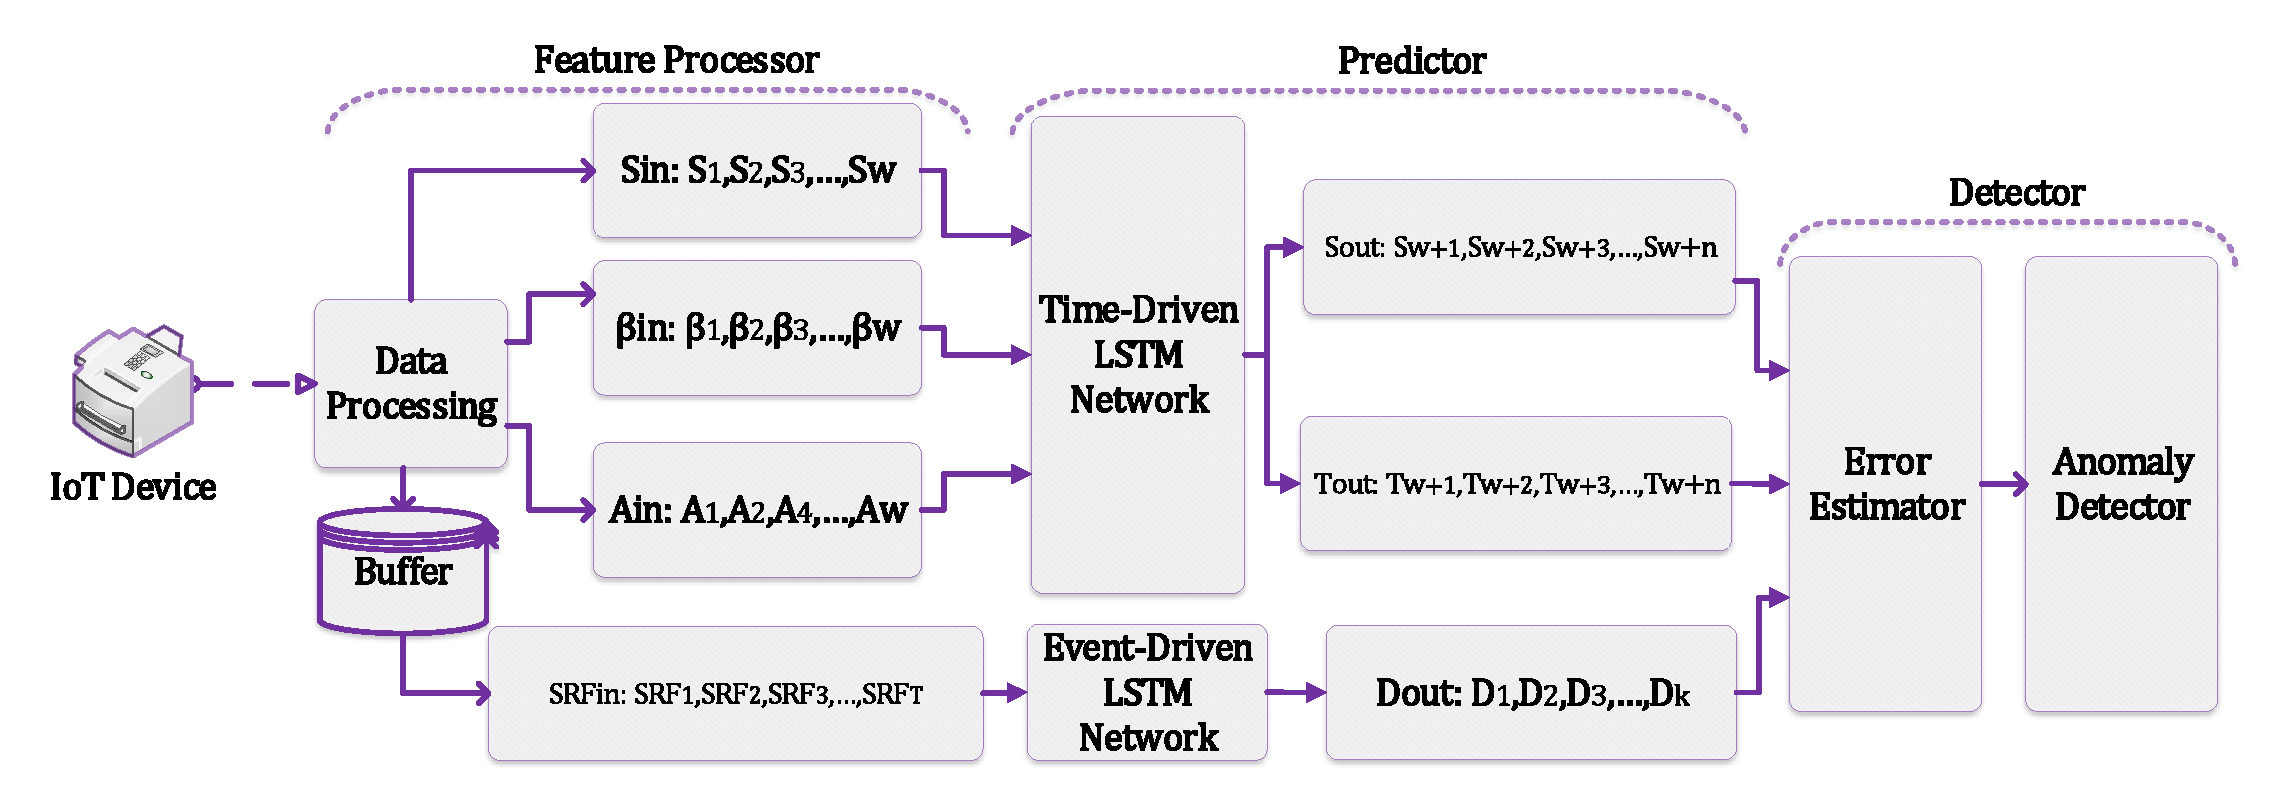
\includegraphics[width=\textwidth, height=7cm]{fpd-model} 
	\caption{Architecture of the Anomaly Model for one IoT Device}
	\label{fig:model-architecture}
\end{figure*} 

\subsubsection{Feature Processor}
\label{subsubsec:preprocessing}
The system call traces contain several properties, but the features of interest 
to us are \emph{timestamp}, \emph{system call ID} and \emph{system call 
	arguments}. To create a relative deterministic model, we avoided using the 
	CPU 
clock or wall clock as a timestamp; alternatively, we use the CPU cycle count. 
We assume that the process is running in a scaled-down operating system with 
not much-competing processes as typically obtained in embedded IoT 
applications. 
Therefore, a single trace is a multivariate variable which undergoes further 
processing to yield the desired features. Given \emph{timestamp} 
as $\mathbf{t} $, system call string name as $ \mathbf{k} $ and system call 
arguments as $ \mathbf{a} $, we process these properties to yield a 
multi-input feature space that we feed to our anomaly models.
\paragraph{Timestamp and System Call Classes}
During the learning phase, we store the training samples in a database, but the 
model runs \emph{online} after learning. Given an observation of system call 
samples $ \lbrace s_1, s_2, 
s_3,\ldots,s_{n} \rbrace $ in storage where $ \bm{n} $ is the 
total number of the observed traces, then the function $ \bm{\beta} $ 
of \eqref{eq:beta} defines the time window between system calls. We target  
both the \emph{ordering} of the system calls and the relative 
\emph{duration} within such a relationship. This way, for malicious code which 
does 
not alter the ordering of the system calls but creates anomalous execution 
times or 
delays which varies from the relative duration defined by 
$\bm{\beta} $ will be labeled a deviation.
\begin{equation}
\bm{\beta}:\left(\bm{t}_i,\bm{t}_{i+1}\right) \longmapsto 
\bm{t}_{i+1} -\bm{t}_i; \; i \in \mathbb{N}  \label{eq:beta}
\end{equation}
To get $ \bm{S} $ in Fig. 
\ref{fig:model-architecture}, we 
use the function defined in \eqref{eq:syscall} to encode the system call strings
into their corresponding Linux tables. There are a total of $ 330 $ unique 
system calls in the $ \verb|X_64| $ platform.
\begin{equation}
\bm{S}: \bm{k} \longmapsto 
\bm{w}; \:
\text{where}\; \bm{w}=\lbrace \mathit{w} \in \mathbb{N} 
\mid 1 \leq \mathit{w} \leq 330 \rbrace 
\label{eq:syscall}
\end{equation}
%\begin{figure}[!t]
%	\centering
%	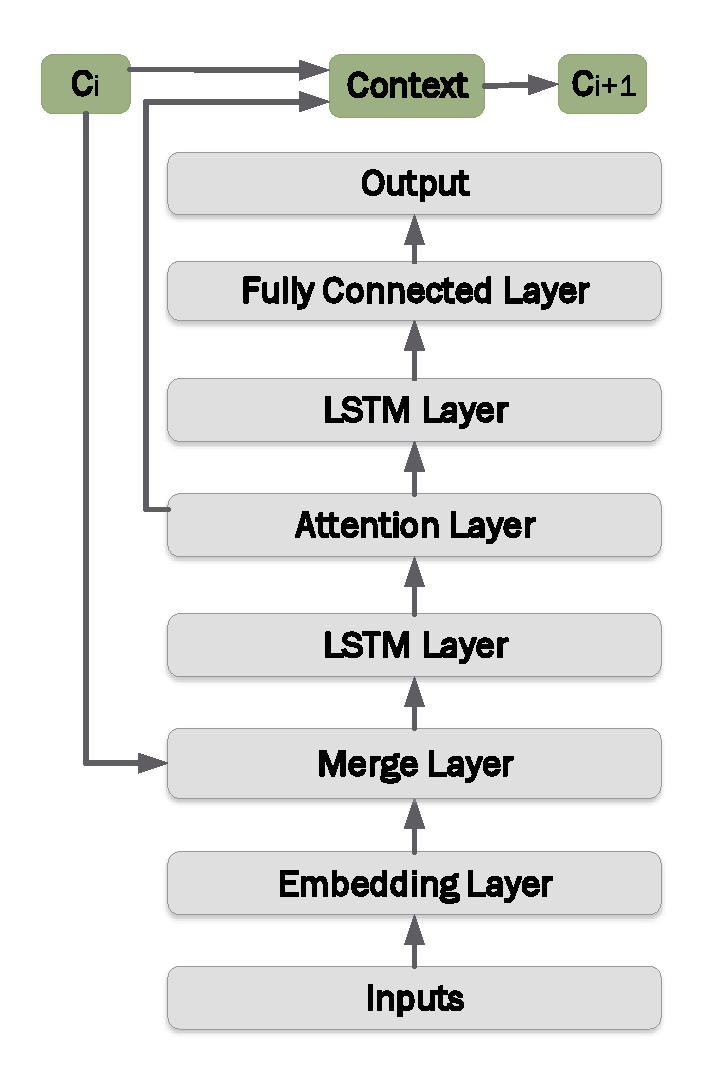
\includegraphics[scale=0.5]{RNN-model}
%	\caption{LSTM-based Design of the Time-Driven and Event-Driven Models }
%	\label{fig:rnn-model}
%\end{figure}
\begin{figure}[!t]
	\centering
	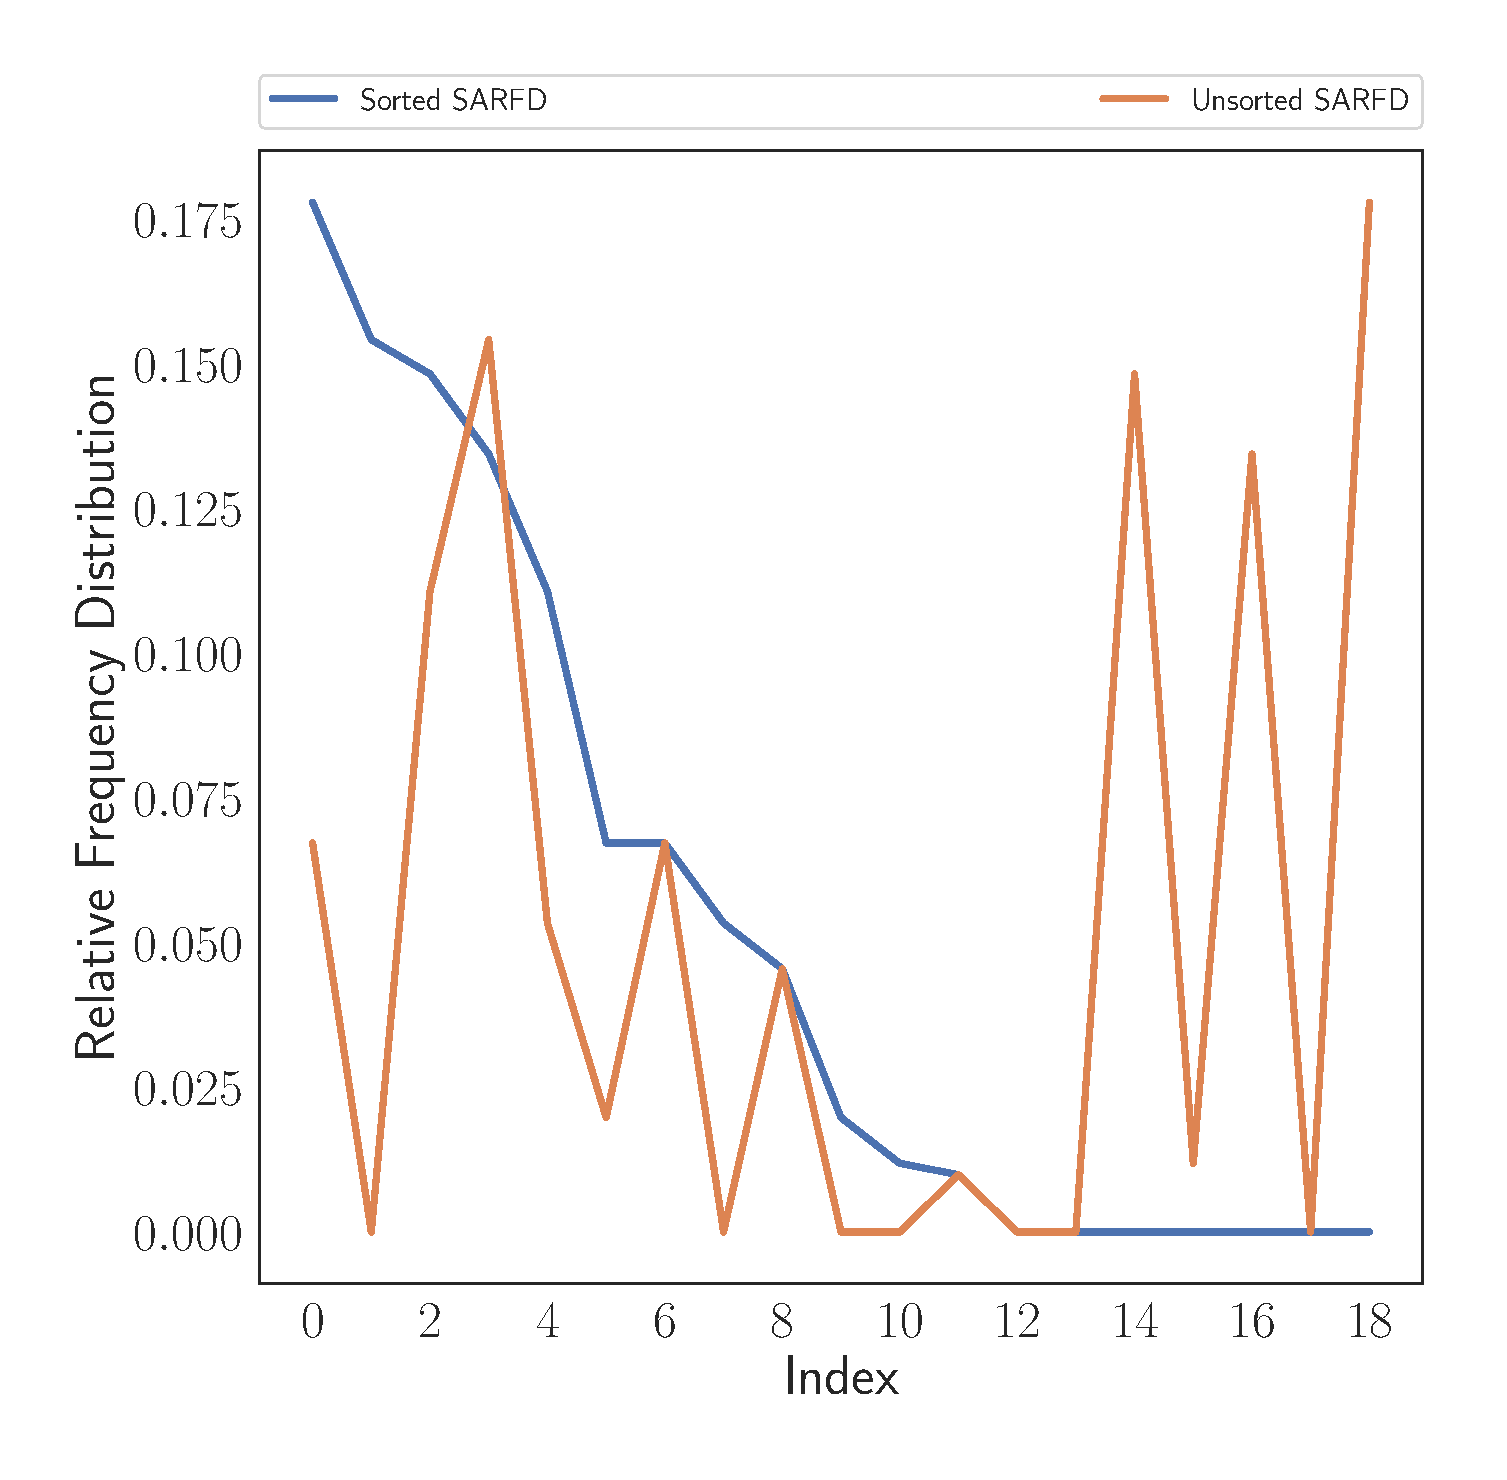
\includegraphics[scale=0.29]{distribution} 
	\caption{Sorted vs Unsorted Relative Frequency Distribution}
	\label{fig:distribution}
\end{figure} 

\paragraph{System Call Arguments}
The system call argument is alphanumeric and special character strings. System 
call arguments are part of the features we process because it has some 
compelling distribution which we use to discriminate between a valid and 
incorrect behavior. The motivation is that while there is no consistent 
frequency distribution in a particular system call, a little reorganization 
(e.g., sorting) of the relative frequency distribution of the characters yields 
a thoughtful insight into its usability. \par
System call arguments are strings, and to maintain a relatively few 
vocabularies, we encode the string characters using \textit{ASCII} values. This 
encoding provides us with a range of unique $\mathbf{256} $ classes. After 
encoding the string values, we calculate the \emph{frequency distribution} and 
\emph{relative frequency distribution} for the $ \bm{256} $ classes in each 
system call argument. 
Our aim is not to check how consistent each \textit{ASCII} value is across the 
system call but to find the \emph{steepness} of the distribution of the 
characters when we sort them. Checking for consistency of each \textit{ASCII} 
value detected during training amounts to assuming that the other characters 
not seen during learning cannot be present in the system call arguments during 
operation, and this is unrealistic. Therefore, we do not consider the kind of 
\textit{ASCII} values present in the argument; we are somewhat concerned about 
the \emph{steepness} of the distribution of the characters per system call. 
Although we do not expect a completely normal distribution, 
legitimate system calls tend to maintain a fairly regular distribution. 
Therefore, we posit that this will improve the model accuracy because 
malicious codes that target the system arguments like \emph{buffer overflow} 
usually stuff the system call arguments with more characters or some 
unprintable characters to achieve their aim. Although tools like 
autocorrelation or Naive Bayes can be used to understand the relationship 
amongst features, these tools learn on the assumptions that each sample is 
independent (thereby lacking temporal relationship), and it focuses on the 
relationship amongst features while we focus on the distribution of the sorted 
\textit{ASCII} values in a sample regardless of the features it contains. \par
To illustrate our point further, let us assume that a system call argument 
returned the following frequency distribution $ \mathbf{x} = 
\left[34,0,56,78,27,10,34,0,23,0,0,5,0,0,75,6,68,0,90\right] $ for $ 
\mathbf{19} $ \textit{ASCII} classes monitored. Then we compute the relative 
frequency distribution ($ \bm{\mathbf{RFD}x_i} $) of one class using $ 
\bm{\mathbf{RFD}_x^i} = \nicefrac{x^i}{\sum_{i=1}^{\abs{x}}} $. Therefore, the 
$ 
\bm{\mathbf{RFD}_x} $ is given as 
[.06,0,.11,...,.13,0,.18]. Now the sorted 
system call argument relative frequency distribution ($ \bm{\mathbf{A}} $) 
of Fig. 
\ref{fig:model-architecture} is the sorted version of $ \bm{\mathbf{RFD}} $. To 
drive home our argument, Fig. \ref{fig:distribution} is a plot of the 
\emph{sorted} $\bm{\mathbf{A}} $ and \emph{unsorted} $\bm{\mathbf{A}} 
$. When we present the unsorted $\bm{\mathbf{A}} $ to a machine learning 
model, it tries to learn the relationship amongst the features at the index of 
the \emph{x-axis}. Therefore, it takes only a structured input whereby the 
index of the incoming features are determined by the class of the feature. On 
the other 
hand, when we present the sorted $\bm{\mathbf{A}} $ to a model, we are 
forcing it to learn how the steepness of the distribution that connects the 
observed classes of the \textit{ASCII} values in a sample without recourse to a 
\emph{fixed index for a particular class}. Therefore, we impose the condition 
of \eqref{eq:A-condition} where $ \bm{\mathbf{n}} $ has a maximum value of 
$ 256 $.
\begin{equation}
\bm{\mathbf{A_{i}}} \geq \bm{\mathbf{A_{i+1}}},\ldots, \geq 
\bm{\mathbf{A_n}} \; 
\text{where}\; \bm{\mathbf{n}} \in \bm{\mathbb{N}}
\label{eq:A-condition}
\end{equation}
Hence, \eqref{eq:A} provides the mapping from the raw string arguments to 
the 
$ \bm{\mathbf{A}} $ feature highlighted in the architecture of Fig. 
\ref{fig:model-architecture}.
\begin{align}
\bm{\mathbf{A}}: \bm{\mathbf{L}} \longmapsto \bm{\mathbf{M}} \; 
\text{where} \label{eq:A} \\
\bm{\mathbf{L}} = \left\lbrace \bm{l \in \mathbb{N} \mid 1 \leq l \leq 256} 
\right\rbrace \\
\bm{\mathbf{M}} = \left\lbrace \bm{m \in \mathbb{R} \mid 0 \leq m \leq 1} 
\right\rbrace \\
\bm{\sum_{i=1}^{256} \mathbf{A}_i = 1}
\end{align}
Also, for every system call encoded with \eqref{eq:syscall}, the 
\emph{data processing} block of Fig. \ref{fig:model-architecture} transmits it 
to the 
\emph{event-driven} lane via the buffer. Then, for every $ 
\nicefrac{F_{TD}}{F_{ED}} $, the system call relative frequency distribution ($ 
\bm{\mathbf{SFR}} $) is computed in the \emph{event-driven} channel as an input 
to the corresponding LSTM network.

\subsubsection{Predictor}
\label{subsec:predictor}
\paragraph{Merge Layer}
Our hypothesis is based on creating a deep execution context via a recursive 
input generated from the attention layer. Since the attention layer has a 
learned weight, it means that its output which is used to create the context $ 
C $ contains information of multiple previous inputs, and feeding it along with 
the present input either reinforces a standard profile or weakens the 
prediction accuracy which will indicate the presence of an anomaly. Therefore, 
\eqref{eq:merge-out} describes our approach of merging the recursive input $ 
\bm{C_i} $ with the present input $ \bm{X_i} $.
\begin{equation}
\bm{v} = \text{merge}(\vec{X_i},\vec{C_i}) \\
\label{eq:merge-out}
\end{equation}

\paragraph{LSTM Layer (Encoder)}
\label{subsec:encoder}
Our choice of LSTM cells in this layer stems from the fact that it is designed 
primarily for time-series data and its recursive nature helps to propagate 
temporal information across so many timesteps infinitely in theory. However, we 
recognize that in practice, there is a limit to how far behind it can propagate 
the errors before the vanishing gradient problem discussed in 
\cite{werbos1990backpropagation} sets in. Hence, our idea to augment it with a 
recursive context to improve the learnability over a long span of time. We 
feed the output of \eqref{eq:merge-out} to the LSTM layer. Different kinds of 
LSTM configuration can be used, but we use the LSTM units described in 
\cite{hochreiter1997long} to create our layer. This layer's output is captured 
mathematically in \eqref{eq:lstm-out}. We omit the bias terms for brevity, and 
$ \bm{\Phi} $ is a nonlinear function like an LSTM. 
\begin{align}
\bm{h}_{i} &= \bm{\Phi}\left(\bm{v}_i,\bm{h}_{i-1} \right)
\label{eq:lstm-out}
\end{align}

\paragraph{Attention Layer}
\label{subsec:attention}
%\begin{figure}[!t]
%	\centering
%	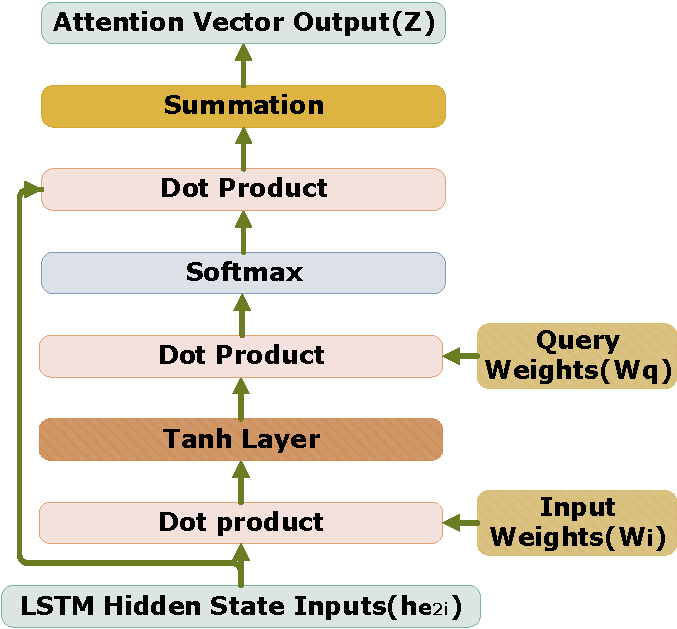
\includegraphics[scale=0.6]{att-layer}
%	\caption{Context-aware Attention Network for the Anomaly Detection Model}
%	\label{fig:att-layer}
%\end{figure}

Differing from \cite{salton2017attentive} that uses memory to create context, 
we add a query weight $\bm{W}_q$ that is learned during training to ensure that 
each tuple is not attended to solely based on the information in the present 
input sequence but also based on the knowledge gained during the learning 
phase. This query performs a similar role as the term-frequency inverse 
document frequency used to weigh the occurrence of tuples in the vector space 
model. The inputs to this layer are the 
input weights $\bm{W}_i$ and the LSTM layer output $\bm{h}_{i} $ of 
\eqref{eq:lstm-out}. We pass the LSTM layer output via a $\tanh$ layer after 
being scaled by the input weights $\bm{W}_i $ and the input bias vector $ 
\bm{b}_i $ to generate correlation vectors $ \bm{m}_i $ given in 
\eqref{eq:m-attention}.

\begin{equation}
\label{eq:m-attention}
\bm{m}_i = \tanh (\bm{W}_{i} \cdot \bm{h}_{i} + \bm{b}_i)
\end{equation}
This correlation vector (\eqref{eq:m-attention}) represents the effect 
of each input based on the present. Hence, we multiply it with the query 
vector $ \bm{W}_q $ which has the \emph{global knowledge} of each input tuple 
in the present input sequence to provide deep horizontally spanning inputs for 
the inference process as shown in \eqref{eq:q-vectors}. This vector is then 
passed through a softmax layer to generate $ \bm{s}_i $ in \eqref{eq:softmax}. 
This normalized value is scaled by the input vectors $ 
\bm{h}_{i}$ and summed to generate the attention vector $ \bm{Z}_i $ in 
\eqref{eq:z-context}.
\begin{align}
\bm{a}_i &= \bm{W}_{q} \cdot \bm{m}_i + \bm{b}_q \label{eq:q-vectors} \\
\bm{s}_i &= \left( \frac{e^{\bm{a}_i}}{\sum_j e^{\bm{a}_j}}\right)_i 
\label{eq:softmax} \\
\bm{Z}_i &= \sum_{i=1}^n \bm{s}_i \times \bm{h}_{i} \label{eq:z-context}
\end{align}

\paragraph{LSTM Layer (Decoder)}
This layer in conjunction with the fully 
connected layer reconstructs the input sequence. This layer creates an 
intermediate output $ \bm{h}_{_di} $ using the previous output $ \bm{y}_{i-1} 
$, the context vector from the attention layer $ \bm{Z} $ and the previous
hidden state $\bm{h}_{_di-1}$ of the previous unit $ d_{i-1} $. Equation 
\eqref{eq:decoder} defines this relationship where $ \Psi $ is a nonlinear 
function called LSTM. Again, bias vector is omitted for brevity.
\begin{align}
\bm{h}_{_di} &= \Psi\left(\bm{h}_{_di-1},\bm{y}_{i-1},\bm{Z}\right) 
\label{eq:decoder}
\end{align}

\paragraph{Fully Connected (Output) Layer}
\label{subsec:decoder}
Our FC layer is a simple dense layer with a dimension matching the expected 
output format. The $ \bm{S_{out}} $ and $ \bm{T_{out}} $ output have the same  
dimension but $ \bm{S_{out}} $ is the number of systems call predicted for $ 
\bm{w} $ number of steps while the $ \bm{T_{out}} $ generates the corresponding 
expected IC for each system call predicted by $ \bm{S_{out}} $. Each of $ 
\bm{S_{out}} $ and $ \bm{T_{out}} $ is represented by \eqref{eq:fc-layer} where 
$ \bm{h}_{_di} $, $ \bm{W}_z $ and $ \bm{b}_z $ are 
the decoder LSTM layer output, the layer weight and the bias vector 
respectively. 
\begin{equation}
\label{eq:fc-layer}
\bm{y}_i = \bm{W}_{z} \cdot \bm{h}_{_di} + \bm{b}_z
\end{equation}
The $ \bm{y}_i $ is further passed through a softmax layer to produce the 
predicted system call $ \mathbf{S}_i $. The whole \emph{predictor} network is 
implemented using the Keras/TensorFlow deep learning tool 
\cite{chollet2015keras}.

\subsubsection{Detector}
\paragraph{Error Estimator}
\label{subsec:error-model}
Given $ \bm{x}_i \in \bm{\mathbb{R}} $ which serves as the input, the target 
during learning is a shifted version $ \bm{x}_{i+w} \in \bm{\mathbb{R}} $ where 
$ \bm{w} $ is the lookahead window. Therefore, the goal is to replicate the 
sequence at the output by creating $ \bm{x}' \in \bm{\mathbb{R}}$. Hence, the 
perfect result is when $\bm{x}_k  \equiv \bm{x}'_k $, but this is hardly 
feasible because of the high randomness caused by interrupts and other events 
in the traces. Hence, when we have $ \bm{f}:\bm{x}\longmapsto \bm{x}' $ given $ 
\bm{x} $ as the ground truths, the deviation $ \bm{d} = \abs{\bm{x} - \bm{x}'} 
$ is the difference between the ground truth and the predicted value for the 
given sequence. This deviation becomes the prediction error values which we 
process further to decide if an anomaly has occurred or not. The anomaly model 
is a \emph{multi-input, multi-output} (MIMO) architecture. Hence, the 
prediction error for the categorical output is the \emph{Boolean error} between 
the predicted and the truth value. While for the regression output, the 
prediction error is the absolute difference between the ground truth and the 
outcome of the prediction.

\paragraph{Anomaly Detector}
\label{subsec:anomaly-detector}
The deviations $ \bm{d}_v = \left\lbrace \bm{d}_1, \bm{d}_2, 
\bm{d}_3,...,\bm{d}_{|V_j|} \right\rbrace  $ from the validation dataset 
constitute random variables which we have no knowledge of the underlying 
distribution. However, since they are error values, we are interested in 
creating an upper bound or threshold in order to capture anomalies. Hence, we 
try to create a threshold value for the prediction errors. Because we know the 
sample $\bm{\mu}$ and variance $\bm{\sigma}^2$,  we employ 
the \emph{Bienaymé-Chebyshev} inequality to compute the threshold. The 
inequality guarantees that no more than a certain fraction of values can be 
more that a certain distance from the $ \bm{\mu} $. The inequality is given in 
\eqref{eq:chebyshev}.
\begin{equation}
\label{eq:chebyshev}
\bm{P}\left(\abs{\bm{X-\mu}} \geq \bm{\Upsilon} \right) \leq 
\frac{\bm{\sigma}^2}{\bm{\Upsilon}^2}
\end{equation}
Although the inequality computes the absolute bound with the assumption of a 
symmetric distribution, we use it in our model because we are only 
interested in the range where the prediction error $ \bm{d} - \bm{\mu} > 1 $. 
Hence, lack of symmetry will not affect the threshold computation. Therefore, 
we interchange $ \bm{\Upsilon} $ in \eqref{eq:chebyshev} with $ 
\abs{\bm{d-\mu}}$ to derive \eqref{eq:chebyshev-2} which we use to compute the 
decreasing probability for increasing deviation $ \abs{\bm{d-\mu}} $ where $ 
\bm{d > \mu} $.
\begin{equation}
\label{eq:chebyshev-2}
\bm{P}\left(\bm{d} > \bm{\mu}\right) = \bm{P}\left(\abs{\bm{X-\mu}} \geq 
\abs{\bm{d-\mu}} \right) = 
\frac{\bm{\sigma}^2}{(\bm{d-\mu})^2}
\end{equation}
One of the advantages that this probability provides is that we do not have to 
know the other parameters of the underlying probability distribution. Also, 
instead of creating a binary threshold of \emph{True} or \emph{False} values, 
this probability gives us an opportunity to quantize the anomaly scores into 
bands per one complete cycle of operation like the safety integrity level 
(\textit{SIL}) provided by safety 
standards like 
\textit{IEC 61508} \cite{bell2006introduction}. Our quantized levels are called 
\emph{anomaly level probability}, ($\bm{AL_p}$) and each level depends on the 
value of the probability from \eqref{eq:chebyshev-2}. As \eqref{eq:chebyshev-2} 
measures how the error values are clustered around the mean, the model is 
expected to create high fidelity predictions (reconstruction of the normal 
profile sequence) to ensure that \eqref{eq:chebyshev-2} performs optimally and 
reduces false negatives.

\subsection{Partition Scheme}
\label{subsec:partition-scheme}
Fig. \ref{fig:distributed-architecture} is the design of our distribut model 
that provides the three core features of \emph{dynamism, scalability} and 
\emph{decentralization} of the anomaly model of Section \ref{subsec:anom-model} 
amongst the local and cloud 
resources. Before we proceed further, it is vital that we explain some of 
the names in Fig. 
\ref{fig:distributed-architecture}. \emph{PUSH, PULL, PUB,} and \emph{SUB} are 
ZeroMQ TCP sockets while \emph{STAGES} $ \bm{1} $ and $ \bm{2} $ represent the 
points where distribution decisions are taken. We use ZeroMQ sockets in our 
design 
because unlike the traditional TCP sockets available in the operating system, 
ZeroMQ sockets pairs can be connected and disconnected arbitrarily in no 
particular order. And this asynchronous behavior removes 
the need of restarting the system if one of the pairs dies and enables the 
partition algorithm to \emph{birth} or \emph{kill} connections on the fly 
during runtime.
\begin{figure}[!t]
	\centering
	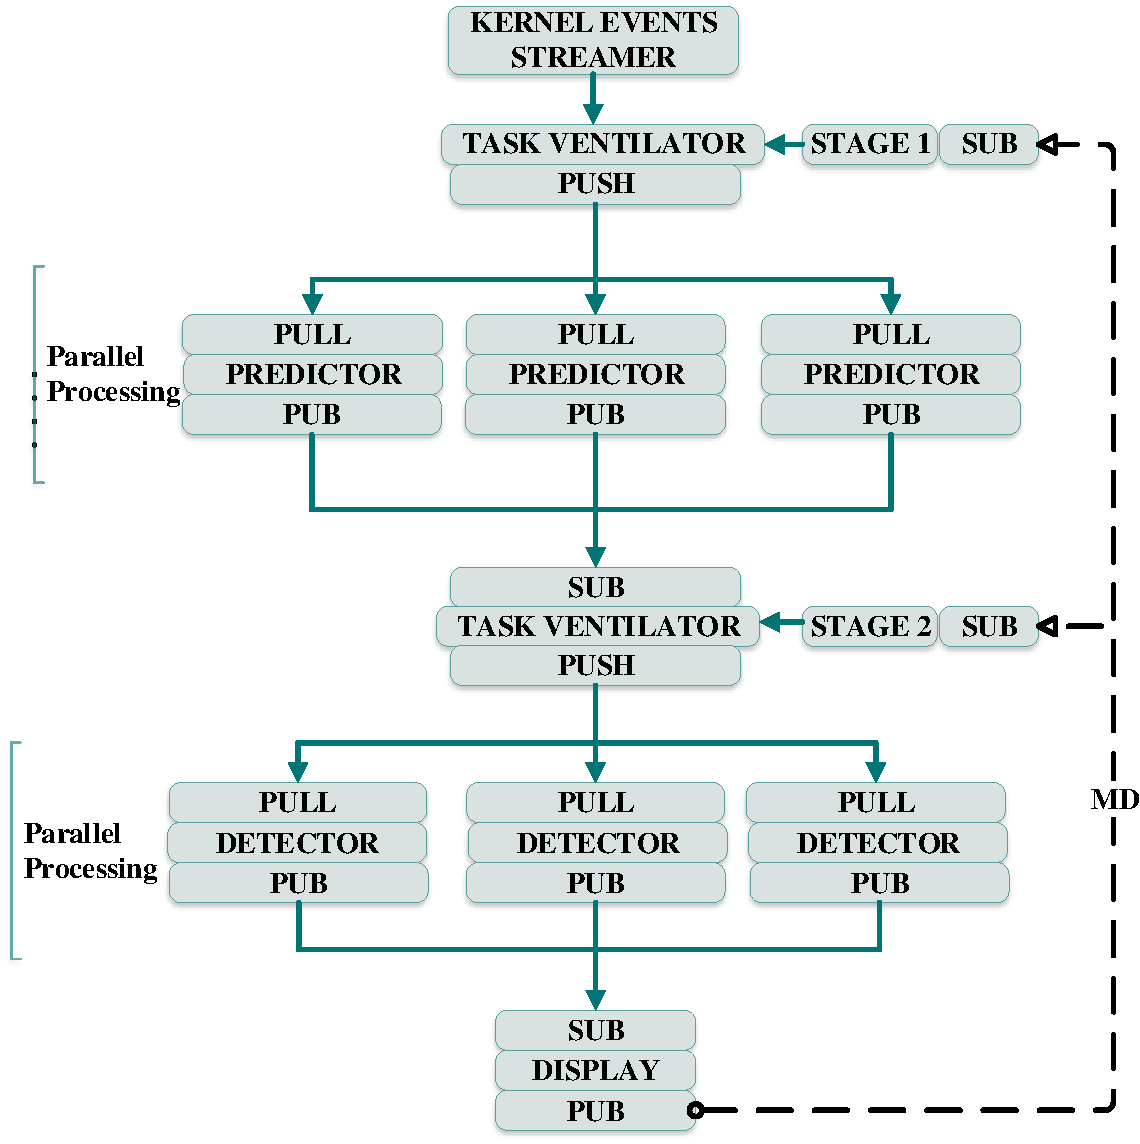
\includegraphics[scale=0.45]{decomposed-model.pdf}
	\caption{D\MakeLowercase{a}SAD Architecture showing the Decentralization 
	and Parallelism}
	\label{fig:distributed-architecture}
\end{figure}
\par
The partitioning scheme works as a data streamer in which the objective is to 
transfer the highest amount of data possible from the \emph{feature processor} 
to the \emph{display} unit of Fig. \ref{fig:distributed-architecture}. 
Therefore, we can represent the scheme as a graph $ 
\bm{G}=\bm{\left(N,P\right)} 
$ where $ \bm{N} = \bm{\lbrace j|j=1,2,3,...,n\rbrace} $ represents the nodes 
\emph{feature processor}, \emph{predictor}, and \emph{detector}, while $ 
\bm{P}=\bm{\lbrace \left(j,k\right)|j,k \in N \rbrace } $ are communication 
paths linking node $ \bm{j} $ to node $ \bm{k} $. Given $ \bm{F}, \bm{P} \; 
\text{and} \; \bm{D}  $ as the \emph{feature processor}, \emph{predictor} and 
\emph{detector} partitions respectively, then, the total time to convey a unit 
of data from $ \bm{F} $ to the \emph{display} is given in \eqref{eq:tot-time}.
\begin{equation}
	\label{eq:tot-time}
	\bm{T_{F,display}}= \bm {\sum_{j}^{n} T_{j,j+1}} \: \forall \bm{j}, \bm{n} 
	\in \bm{N}
\end{equation}
Note that $ \bm{n} $ denotes the detector node in \eqref{eq:tot-time}. \par
The constraints in our partitioning scheme modeling are: \emph{communication 
bandwidth} between nodes $ \bm{B} $, free \emph{local system resource} $ 
\bm{R_s} $, the \emph{energy level} $ \bm{E_l} $ of the IoT device and the 
system resource needed by the node application at that partition $ \bm{Ra} $.   
Therefore, $ \bm{T_{j,j+1}} =   $
With so many frivolous properties logged  during the kernel tracing, and a  
constrained transmission bandwidth, compute and memory resources as well 
as energy, the partition scheme determines the 
 
\paragraph{Feature Processor}
\label{subsec:process-stage1}
The \emph{feature processor} handles the processing of 
the kernel events emanating from the instrumented kernel as described in 
Section \ref{subsubsec:preprocessing}. As we mentioned in 
Section \ref{sec:introduction}, we only process the attributes which are common 
across the trace irrespective of the system to remove any system-induced bias 
on the classifier. In kernel, an 
example event stream of $\text{open} \longrightarrow \text{mmap} 
\longrightarrow \text{close} \longrightarrow \text{read}$ has 
\emph{timestamps, PID, TID, NID}, etc. which are common across the event 
stream. Therefore, we formulate the characteristics of interest using these 
features which exist across kernel event streams irrespective of platform. 


%\subsubsection*{Task Ventilation}
%\label{subsub:task1}
%The frequency of the kernel event streamer is high, and the downstream modules 
%have to keep up with the streams in order to avoid the sockets dropping the 
%data. Hence, the need for parallelism at the \emph{predictor}. As stated in 
%Section \ref{sec:design}, the sockets can connect and disconnect arbitrarily 
%without restarting the network thereby providing an efficient horizontal 
%scaling mechanism for the parallel predictors and detectors. Our dynamic 
%allocation scheme starts in \eqref{eq:new-pred-num} where we determine the 
%number of new predictors $ \bm{N_p} $ we can create locally using the free 
%system resources (compute and memory) $ \bm{R_{s}} $, the energy level $ 
%\bm{E_l} $ of the embedded device and the system resources $ \bm{R_p} $ 
%required by a predictor. 
%
%\begin{align}
%\label{eq:new-pred-num}
%\bm{N_p} &= \bm{\frac{R_{s}\times E_{l}}{R_{p}}} \\
%\label{eq:total-pred-local}
%\bm{\tau_{p}} &= \bm{N_p + N_{local}}
%\end{align}
%The total number of predictors that we can run on the embedded device is given 
%in \eqref{eq:total-pred-local} pending the outcome of conditions 
%\eqref{eq:PI-local} and \eqref{eq:PI-cloud}. $ \bm{N_{local}} $ of 
%\eqref{eq:total-pred-local} refers to already running instances of predictors 
%on the embedded device.
%\begin{align}
%	\label{eq:PI-local}
%	\bm{PI_{local}} & = \bm{\frac{\tau_{p}}{C_p\times F_k}} \\
%	\label{eq:PI-cloud}
%	\bm{PI_{cloud}} &= \bm{\frac{TDD_1}{PI_{local}\times \lambda}}\; 
%	\text{where} \; \lambda \ge 1
%\end{align}
%To determine the performance of the predictors locally and in the cloud, we 
%use 
%\eqref{eq:PI-local} and \eqref{eq:PI-cloud} which we refer to as the local 
%(embedded device) and cloud performance index (PI) respectively. $ \bm{C_p} $ 
%and $ 
%\bm{F_k} $ refers to the computational time of the predictor in seconds and 
%the 
%kernel event streamer frequency which is measured in input/seconds. In 
%\eqref{eq:PI-cloud}, $ \bm{\lambda} $ is the speed factor we get for 
%processing 
%in the cloud and $ \bm{TDD_1} $ is the total delay from the ventilator to the 
%display when the predictors in the cloud are used. The metadata feedback loop 
%of Fig. \ref{fig:distributed-architecture} provides the $ \bm{TDD_1} $ 
%information. For every task sent to the cloud from the stage 1 ventilator, the 
%cloud detector is equally used for anomaly detection and the result published 
%to the display. In our model, there is no automatic system reaction to the 
%detection of an anomaly; hence we envisage the display to be operated by a 
%human operator. Therefore, the display is assumed to be in the monitoring 
%room. 
%The SUB sockets of the stage 2 task ventilator and the display provide the 
%metadata information on the number of parallel predictors and detectors 
%running 
%locally via the metadata (MD) feedback loop.
%Now, examining \eqref{eq:PI-local} and \eqref{eq:PI-cloud} closely, we see 
%that 
%they vary inversely to one another. So, as the streaming frequency $ \bm{F_k} 
%$ 
%increases compared to the available number of predictors, the local 
%performance 
%index $ \bm{PI_{local}} $ decreases and the cloud performance index $ 
%\bm{PI_{cloud}} $ increases, thereby favoring more predictors to be run in the 
%cloud and vice versa. Therefore, \eqref{eq:new-pred-num} to 
%\eqref{eq:PI-cloud} 
%create a \emph{self-scalable} and \emph{distributed} system for handling both 
%the predictor and detector tasks. The latency requirement of the application 
%places a bound on the viable values of $ \bm{TDD_1} $ that is permissible in 
%the model.
%
%\subsection{Predictor}
%\label{subsec:predictor}
%\subsubsection*{Merge Layer}
%Our hypothesis is based on creating a deep execution context via a recursive 
%input generated from the attention layer. Since the attention layer has a 
%learned weight, it means that its output which is used to create the context $ 
%C $ contains information of multiple previous inputs, and feeding it along 
%with 
%the present input either reinforces a standard profile or weakens the 
%prediction accuracy which will indicate the presence of an anomaly. Therefore, 
%\eqref{eq:merge-out} describes our approach of merging the recursive input $ 
%\bm{C_i} $ with the present input $ \bm{X_i} $.
%\begin{equation}
%\bm{v} = \text{merge}(\bm{\vec{X_i},\vec{C_i}}) \\
%\label{eq:merge-out}
%\end{equation}
%
%\subsubsection*{Encoder (LSTM Layer)}
%\label{subsubsec:encoder}
%Our choice of LSTM cells in this layer stems from the fact that it is designed 
%primarily for time-series data and its recursive nature helps to propagate 
%temporal information across so many timesteps infinitely in theory. However, 
%we 
%recognize that in practice, there is a limit to how far behind it can 
%propagate 
%the errors before the vanishing gradient problem sets in. Hence, our idea to 
%augment it with a 
%recursive context to improve the learnability over a long span of time. We 
%feed the output of \eqref{eq:merge-out} to the LSTM layer. Different kinds of 
%LSTM configuration can be used, but we use the LSTM units described in 
%\cite{hochreiter1997long} to create our layer. This layer's output is captured 
%mathematically in \eqref{eq:lstm-out}. We omit the bias terms for brevity, and 
%$ \bm{\Phi} $ is a nonlinear function like an LSTM. 
%\begin{align}
%\bm{h}_{i} &= \bm{\Phi}\left(\bm{v}_i,\bm{h}_{i-1} \right)
%\label{eq:lstm-out}
%\end{align}
%
%\subsubsection*{Attention Layer}
%\label{subsubsec:attention}
%Differing from \cite{salton2017attentive} that uses memory to create context, 
%we add a query weight $\bm{W}_q$ that is learned during training to ensure 
%that 
%each tuple is not attended to solely based on the information in the present 
%input sequence but also based on the knowledge gained during the learning 
%phase. This query performs a similar role as the term-frequency inverse 
%document frequency used to weigh the occurrence of tuples in the vector space 
%model. The inputs to this layer are the 
%input weights $\bm{W}_i$ and the LSTM layer output $\bm{h}_{i} $ of 
%\eqref{eq:lstm-out}. We pass the LSTM layer output via a $\tanh$ layer after 
%being scaled by the input weights $\bm{W}_i $ and the input bias vector $ 
%\bm{b}_i $ to generate correlation vectors $ \bm{m}_i $ given in 
%\eqref{eq:m-attention}.
%
%\begin{equation}
%\label{eq:m-attention}
%\bm{m}_i = \tanh (\bm{W}_{i} \cdot \bm{h}_{i} + \bm{b}_i)
%\end{equation}
%
%The correlation vector \eqref{eq:m-attention} represents the effect 
%of each input based on the present. Hence, we multiply it with the query 
%vector $ \bm{W}_q $ which has the \emph{global knowledge} of each input tuple 
%in the present input sequence to provide deep horizontally spanning inputs for 
%the inference process as shown in \eqref{eq:q-vectors}. This vector is then 
%passed through a softmax layer to generate $ \bm{s}_i $ in \eqref{eq:softmax}. 
%This normalized value is scaled by the input vectors $ 
%\bm{h}_{i}$ and summed to generate the attention vector $ \bm{Z}_i $ in 
%\eqref{eq:z-context}.
%\begin{align}
%\bm{a}_i &= \bm{W}_{q} \cdot \bm{m}_i + \bm{b}_q \label{eq:q-vectors} \\
%\bm{s}_i &= \left( \frac{e^{\bm{a}_i}}{\sum_j e^{\bm{a}_j}}\right)_i 
%\label{eq:softmax} \\
%\bm{Z}_i &= \sum_{i=1}^n \bm{s}_i \times \bm{h}_{i} \label{eq:z-context}
%\end{align}
%
%\subsubsection*{Decoder (LSTM Layer)}
%This layer performs the function of a decoder while the lower LSTM is 
%responsible for encoding the input. This layer in conjunction with the fully 
%connected layer tries to reconstruct the input sequence. This layer creates an 
%intermediate output $ \bm{h}_{_di} $ using the previous output $ \bm{y}_{i-1} 
%$, the context vector $ \bm{Z} $ and the previous
%hidden state $\bm{h}_{_di-1}$ of the previous unit $ d_{i-1} $. Equation 
%\eqref{eq:decoder} defines this relationship where $ \Psi $ is a nonlinear 
%function called LSTM. Again, bias vector is omitted for brevity.
%\begin{align}
%\bm{h}_{_di} &= \Psi\left(\bm{h}_{_di-1},\bm{y}_{i-1},\bm{Z}\right) 
%\label{eq:decoder}
%\end{align}
%
%\subsubsection*{Output Layer}
%\label{subsubsec:decoder}
%Our output layer is a simple dense layer with same number of units as there 
%are 
%unique features in the input sequences. The output of this layer is given in 
%\eqref{eq:fc-layer} where $ \bm{h}_{_di} $, $ \bm{W}_z $ and $ \bm{b}_z $ are 
%the decoding LSTM layer output, the layer weight and the bias vector 
%respectively. 
%\begin{equation}
%\label{eq:fc-layer}
%\bm{y}_i = \bm{W}_{z} \cdot \bm{h}_{_di} + \bm{b}_z
%\end{equation}
%The $ \bm{y}_i $ is then passed through a softmax layer to produce the 
%predicted system call $ \mathbf{S}_i $. 
%
%
%\subsection{Stage 2 Ventilator Module}
%\label{subsec:stage2}
%We apply the stage 1 ventilator equations of Section \ref{subsec:stage1} to 
%determine how we distribute the detectors but $ \bm{TDD_2} $ replaces $ 
%\bm{TDD_1} $ and reference symbol is now the detector $ \bm{d} $ and not the 
%predictor $ \bm{p} $. 
%\subsection{Detector}
%\label{subsec:detector}
%\subsubsection*{Error Estimator and Anomaly Detection}
%\label{subsec:error-model}
%Given $ \bm{x}_i \in \bm{\mathbb{R}} $ which serves as the input, the target 
%during learning is a shifted version $ \bm{x}_{i+w} \in \bm{\mathbb{R}} $ 
%where 
%$ \bm{w} $ is the lookahead window. Therefore, the goal is to replicate the 
%sequence at the output by creating $ \bm{x}' \in \bm{\mathbb{R}}$. Hence, the 
%perfect result is when $\bm{x}_k  \equiv \bm{x}'_k $, but this is hardly 
%feasible because of the high randomness caused by interrupts and other events 
%in the traces. Hence, when we have $ \bm{f}:\bm{x}\longmapsto \bm{x}' $ given 
%$ 
%\bm{x} $ as the ground truths, the deviation $ \bm{d} = \abs{\bm{x} - \bm{x}'} 
%$ is the difference between the ground truth and the predicted value for the 
%given sequence. This deviation becomes the prediction error values which we 
%use 
%to to fit a non-parametric kernel density estimator. The output of the 
%estimator is clustered with k-means clustering where $ \bm{k=2} $.

\subsection{Display}
\label{subsec:display}
We send the clustering decision to the display via the PUB sockets of the 
detector. The display extracts the metadata information and relays the same to 
stages 1 and 2. Information from the display can also be used for corrective 
actions when an anomaly is detected. 


\section{Experimental Evaluation}
\label{sec:experiments}
\subsection{Dataset}
\begin{figure}[!t]
	\centering
	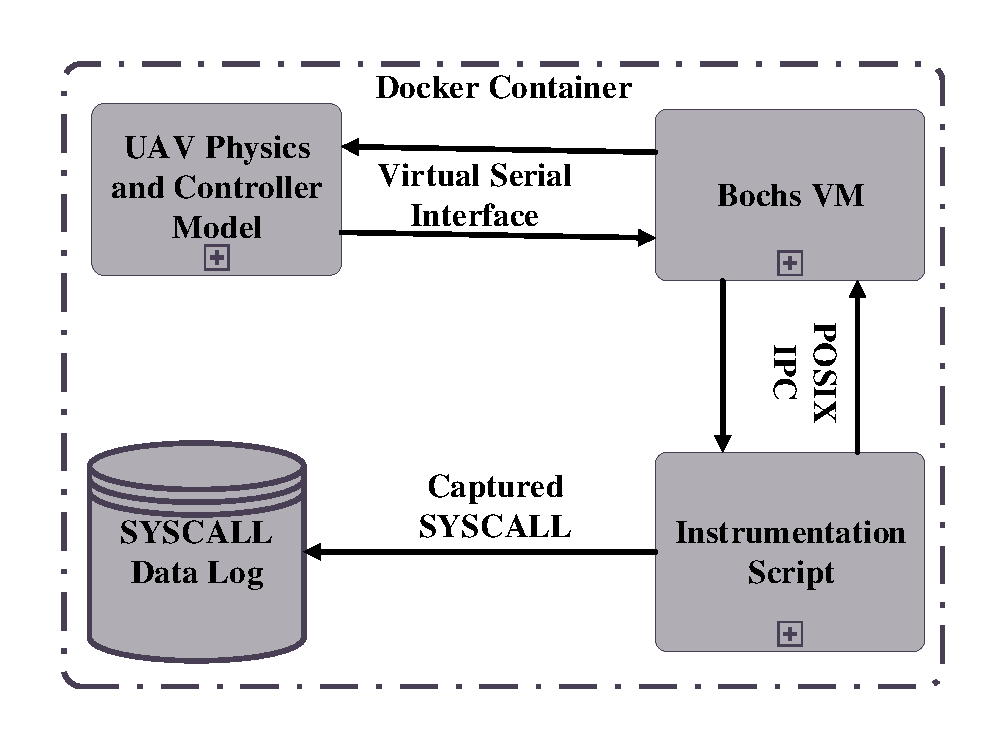
\includegraphics[scale=0.5]{dataset-experimental-setup}
	\caption{Setup of the Experiment for Dataset Generation}
	\label{fig:setup}
\end{figure}

\begin{figure}[!t]
	\centering
	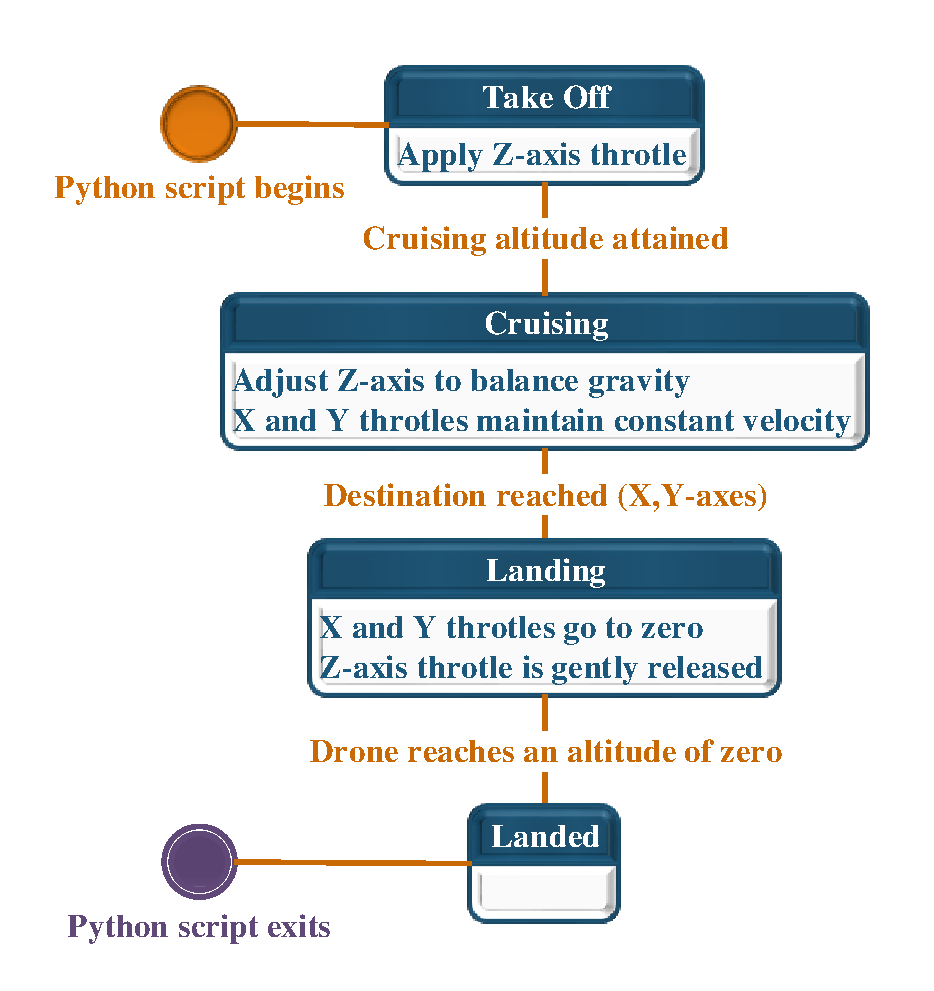
\includegraphics[scale=0.5]{FSM-drone}
	\caption{State Machine Diagram of the UAV Controller}
	\label{fig:FSM}
\end{figure}
We use the publicly available kernel event dataset of \cite{salem2016anomaly} 
to test our model. According to the authors in \cite{salem2016anomaly}, the 
\emph{hilRf-InFin} scenario corresponds to the default system setting while 
\emph{full-while} scenario refers to generating fictitious tasks via a while 
loop to waste CPU resources by competing for the same CPU resource with the 
standard tasks running the UAV. The \emph{fifo-ls} and \emph{sporadic} 
situations derive their names from the scheduling algorithms in the operating 
system and are identified by the corresponding scheduling algorithm used in 
each experiment. 
\subsection{Experimental Setup and Networking}
Our testbed constitutes of Raspberry PI 3 platform which serves as our local 
embedded device and an Intel-i5 laptop which serves as our cloud. Each of the 
scenarios in the dataset has a separate model, and our 
experimental objectives are:
\begin{enumerate*}[label={\alph*)},font={\bfseries}]
	\item demonstrate the offloading mechanism which creates a self-scaling and 
	a distributed model.  
	\item demonstrate the improvement brought by the attention layer to the 
	anomaly model by comparing with a \emph{base} (no attention layer) model.
\end{enumerate*}
We implement our model of Fig. \ref{fig:distributed-architecture} using ZeroMQ 
\cite{Akgul:ZEROMQ}. First, the predictor and detector model weights are loaded 
in both the Raspberry PI and the laptop computer which serves as our 
cloud. Our sockets does not have restrictions on which end \emph{binds} and 
which end \emph{connects}. Therefore, it our design decision that any 
\emph{one-to-many} connection like that of \emph{stage 1 task ventilator PUSH} 
socket and \emph{predictor PULL} sockets, \emph{stage 2 task ventilator PUSH} 
and \emph{detector PULL} sockets, we bind the \emph{one} and connect the 
\emph{many}. This way, the PULL socket processes in the predictor and detector 
can be scaled up and down without affecting the network functionality since 
ZeroMQ permits arbitrary 
\emph{connect} and \emph{disconnect}. For the \emph{many-to-one} connection of 
the \emph{predictor PUB} and the \emph{stage 2 task ventilator SUB}, 
\emph{detector PUB} and \emph{display SUB}, we bind the \emph{one} and connect 
the \emph{many} as well. The \emph{PUSH-PULL} sockets provide 
\emph{parallelism} while the \emph{PUB-SUB} sockets act as \emph{source-sink} 
connection. The metadata \emph{MD} feedback loop implemented with a 
\emph{PUB-SUB} connection carries 
information about the active number of predictors and detectors as well as the 
$ \bm{TDD_1} 
$ and $ \bm{TDD_2} $ delay.
\subsection{Results}
\subsubsection{Offloading Mechanism Results}
To test the offloading mechanism, we vary the number of running processes in 
the Raspberry PI from nearly idle to near full utilization of the CPU and 
memory. We fixed the maximum number of predictors and detectors that can be run 
both in the cloud and the embedded device using \eqref{eq:total-pred-local}. 
Then, we allow the offloading mechanism to use the interaction between the $ 
\bm{PI_{local}} $ and $ \bm{PI_{cloud}} $ to generate the cloud and local 
performance index as the system gets busier. The number of local detectors and 
predictors running in a particular platform is directly proportional to its 
performance index $ \bm{PI} $. In Fig. \ref{fig:PI-plot}, we plot the $ \bm{PI} 
$ of the \emph{local} (embedded system) versus the \emph{cloud} platform. We 
place the Raspberry PI in the same network as the laptop and also experiment 
with both of the devices in different networks. In both cases, the patterns of 
the $ \bm{PI} $ plot is the same except for a slow rise time of the $ 
\bm{PI_{cloud}} $ when the $ \bm{TDD} $ is high due to network congestion. We 
determine the maximum $ \bm{TDD} $ based on heuristic when there is mild 
traffic in the network as $\bm{TDD}  = \bm{p_d+t_d+p_t}$  where $\bm{p_d}$ is 
the \emph{propagation 
delay}, $\bm{t_d}$ is the \emph{transmission delay} and $\bm{p_t}$ is the 
\emph{processing time} at the cloud.
\begin{figure}[!t]
	\centering
	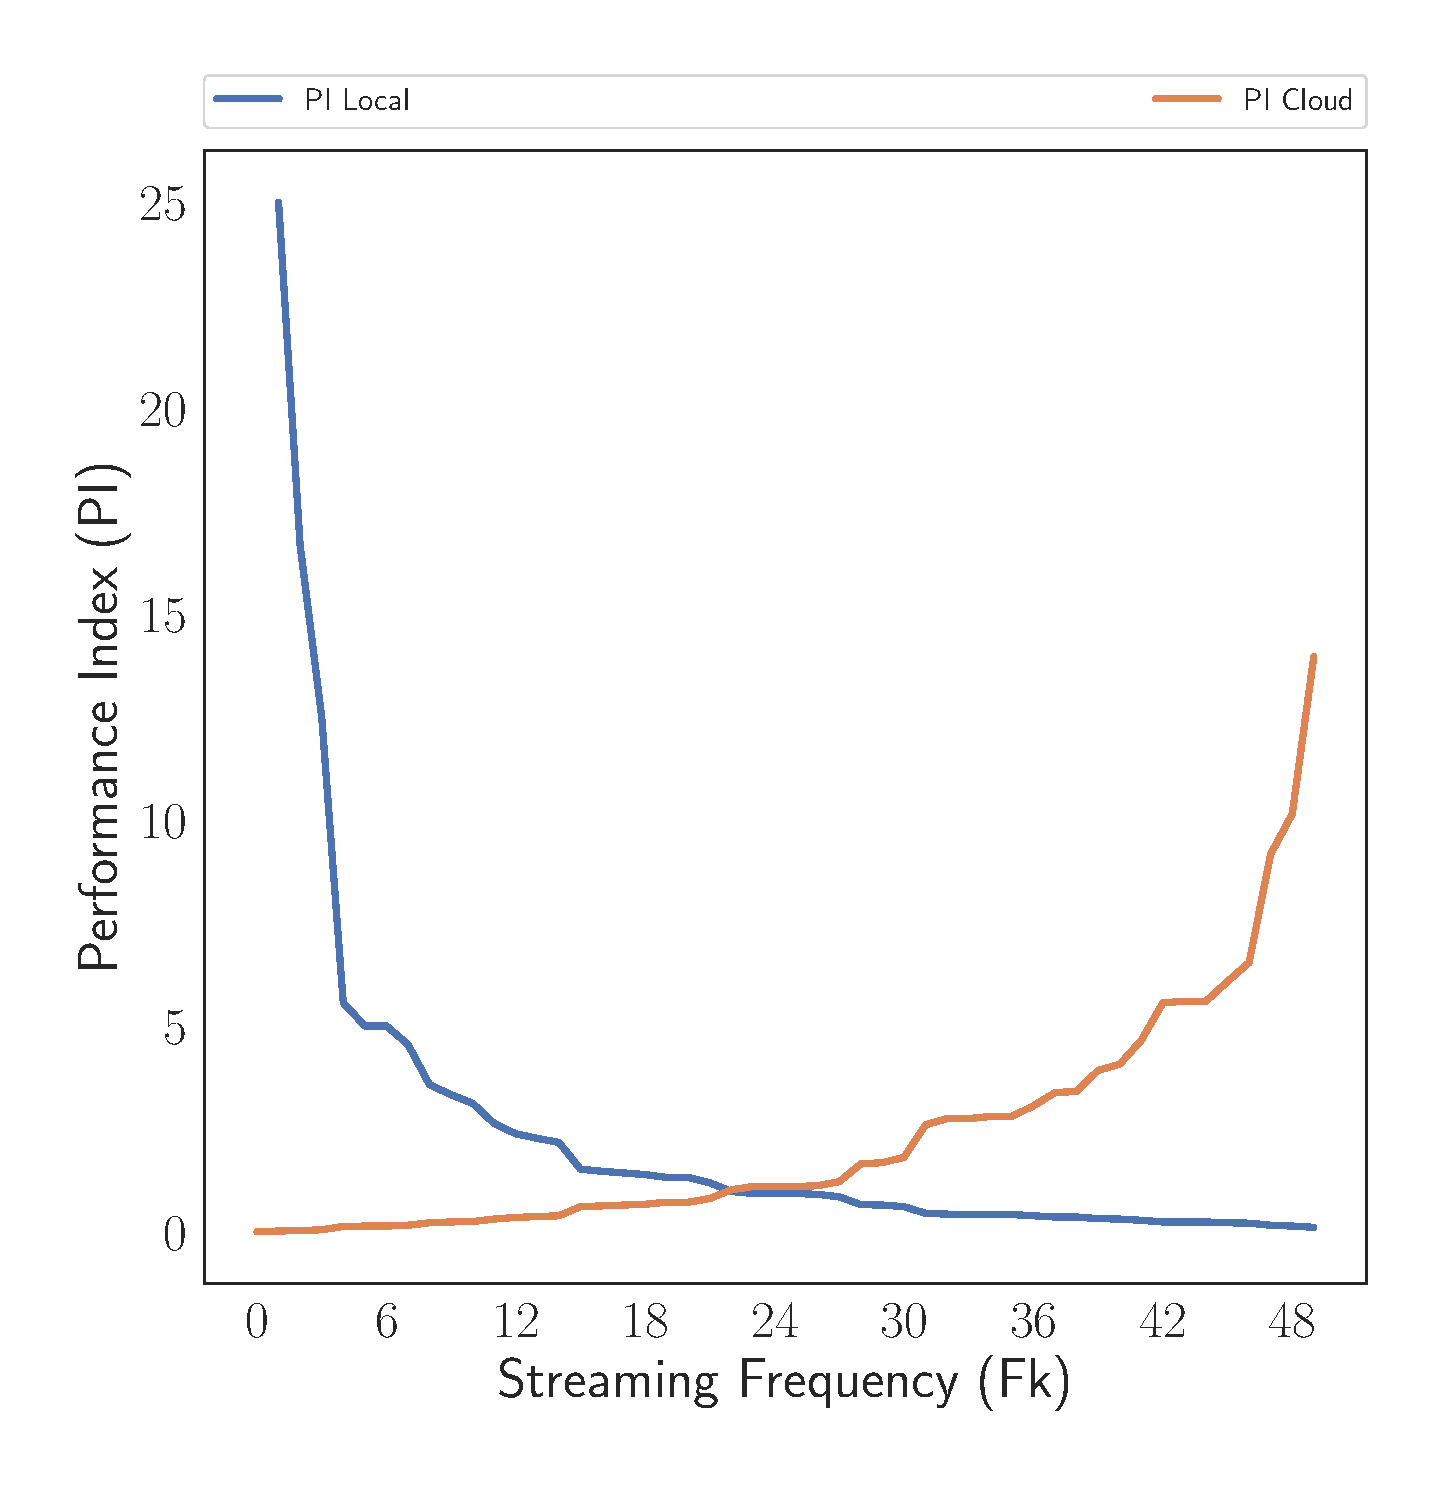
\includegraphics[scale=0.37]{performance-index.pdf} 
	\caption{Performance Index $ \bm{PI} $ of the Cloud and Embedded (Local)  
	Platform versus Streaming Frequency $ \bm{F_k} $}
	\label{fig:PI-plot}
\end{figure}
\begin{table}[!t]
	\renewcommand{\arraystretch}{1}
	\caption{Accuracy of Attention-Based Model vs the Base Model with Varying $ 
	\bm{\Phi_i} $}
	\label{tab:model-results}
	\centering
	\begin{tabu} to 0.49\textwidth {|X[l]|X[c]|X[c]|X[c]|X[c]|}
		\hline
		Experiment & Models & \multicolumn{3}{|c|}{Lookahead Window Accuracy} \\
		\hline
		& &$ \Phi_{1} $&$ \Phi_{5} $&$ \Phi_{10} $ \\
		\cline{1-5}
		\multirow{3}{*}{fifo} & Base & $ 0.794 $ & $ 0.746 $ & $ 0.724 $ \\
		\cline{2-5}
		& Att-Model & $ 0.981 $ & $ 0.972 $ & $ 0.947 $ \\
		\hline 
		\multirow{2}{*}{full}& Base & $ 0.836 $ & $ 0.791 $ & $ 0.767 $ \\
		\cline{2-5}
		& Att-Model & $ 0.99 $ & $ 0.942 $ & $ 0.916 $  \\
		\hline 
		\multirow{2}{*}{hilrf}& Base & $ 0.870 $ & $ 0.815 $ & $ 0.778 $ \\
		\cline{2-5}
		& Att-Model & $ 0.968 $ & $ 0.937 $ & $ 0.908 $ \\
		\hline
		\multirow{2}{*}{sporadic}& Base & $ 0.790 $ & $ 0.772 $ & $ 0.728 $  \\
		\cline{2-5}
		& Att-Model & $ 0.916 $ & $ 0.872 $ & $ 0.857 $ \\
		\hline 
	\end{tabu}
\end{table}
\subsubsection{Base Model vs Attention-based Model Results}
\label{subsec:att-vs-noatt}
With high input frequency rate, we varied the lookahead window to reduce the 
number of iterations that we run the predictor and the detector and conserve 
the embedded system resources. While this conserves resources, its 
effectiveness depends on the accuracy of our model. We represent the ratio of 
the input stream window to the output lookahead window as $ \bm{\Phi} = 
\nicefrac{\theta_{in}}{\theta_{out}} $. Therefore, $ \bm{\Phi_{i}} $ is the 
\emph{input-output} window ratio for lookahead length $ \bm{i} $. We use early 
stopping and dynamic learning rate during training to control the number of 
training epochs and improve the performance of the \emph{adam} 
\cite{kingma2014adam} optimization scheme that was used during the training 
process. In Table \ref{tab:model-results}, two patterns emerge:
\begin{enumerate*}[label={\alph*)},font={\bfseries}]
	\item the attention-based model we designed consistently outperforms the 
	base model in every $ \bm{\Phi_i} 
	$.
	\item there is decreasing accuracy as we increase $ \bm{i} $ in $ \bm{\Phi} 
	$. 
\end{enumerate*}
These patterns conform with our postulation that the attention layer and the 
recursive input of of the model impact positively on the model performance. 
Also, with a fixed input window, $ \theta_{in} $, the decreasing accuracy with 
increasing $ \theta_{out} $ is expected as the temporal information needed for 
longer sequence generation is restricted.

\section{Conclusions and Future Work}
\label{sec:conclusion}
We propose a dynamic, distributed and self-scaling anomaly detection model 
targeting resource-constrained embedded devices. We detail the implementation 
of the model as well as the hypothesis behind the model design. Our 
experimental results validate our hypothesis on the offloading scheme. Also, 
the postulation of creating a recursive-context using the attention layer is 
confirmed as shown in the results. Finally, while our model can be deployed for 
\emph{soft} real-time systems, we will be exploring more robust offloading 
schemes for \emph{hard} real-time embedded applications so that the $ TDD $ 
bounds are based on real-time application's latency requirement.

\bibliographystyle{ACM-Reference-Format}
\bibliography{lctes}

\end{document}
